\documentclass{scrartcl}
\usepackage[inner=3cm,top=2.5cm,outer=3.5cm]{geometry}
% \usepackage{fontspec} 
% \defaultfontfeatures{Mapping=tex-text}
% \setromanfont [Ligatures={Common}, Numbers={OldStyle}]{Hoefler Text}
% \setmonofont[Scale=MatchLowercase]{Inconsolata} 
% \setsansfont[Scale=MatchLowercase]{Optima Regular} 

\usepackage[utf8]{inputenc}
\usepackage{graphicx}
\DeclareGraphicsExtensions{.png,.pdf}
\usepackage{hyperref}
\usepackage{color}
\definecolor{slateblue}{rgb}{0.07,0.07,0.488}
\hypersetup{colorlinks=true,linkcolor=slateblue,anchorcolor=slateblue,citecolor=slateblue,filecolor=slateblue,urlcolor=slateblue,bookmarksnumbered=true,pdfview=FitB}
\usepackage{url}
\usepackage[round,sectionbib]{natbib}
\bibliographystyle{abbrvnat}
\usepackage[small]{caption}
\usepackage[small]{titlesec}
\usepackage{slashbox}
\usepackage{booktabs}
\usepackage{alltt}
\usepackage{listings}
\lstset{
  basicstyle=\ttfamily,
}
\newcommand{\code}[1]{\lstinline!#1!}
\newcommand{\f}[1]{\lstinline!#1()!}
\usepackage{xspace}
\newcommand{\plyr}{{\tt plyr}\xspace}
\newcommand{\x}{\,$\times$\,}

\usepackage{multicol}
\setlength\columnseprule{.4pt}
\setlength{\columnsep}{2pc}

\title{plyr: divide and conquer}
\author{Hadley Wickham}
\begin{document}
\maketitle

% SET_DEFAULTS
%   GG-WIDTH: 4  GG-HEIGHT: 4
%   TEX-WIDTH: 0.5\textwidth
%   INLINE: FALSE
%   CACHE: TRUE
%

% END

\begin{abstract}
plyr is a set of tools for a common set of problems: you need to break a big problem down into manageable pieces, operate on each pieces and then put all the pieces back together.  I call this strategy ``split-apply-combine'' and the three components form..   This paper describes the components that make up plyr.  It includes two case studies.
\end{abstract}

\section{Introduction}

The {\tt plyr} package provides tools for solving a common class of problems, where you break apart a big complicated data structure into small simple pieces, operate on each piece independently and then put all the pieces back together (possibly in a different format to the original).  This paper introduces the {\tt ply} family of functions which generalise the {\tt apply} family found in the base package, and include all combinations of input and output of lists, data frames and arrays.

This paper describes version 0.1 of {\tt plyr}, which requires R 2.7.0 or later and has no run-time dependencies.  To install it from within R, run {\tt install.packages("plyr")}.  Information about the latest version of the package can be found online at \url{http://had.co.nz/plyr}.  

% If you have any questions or comments about {\tt plyr}, please feel free to email me directly at \href{mailto:h.wickham@gmail.com}{h.wickham@gmail.com}.

In general, plyr provides a replacement for for loops for a large set of practical problems.  The major assumption that the {\tt ply} functions make is that each piece can be operated on independently of the other pieces, so if there is any dependence between the pieces then you will need to use other tools.  The need to provide an alternative to loops does not come about because loops are slow (they are not!), but because they do not clearly express the intent of the algorithm, as important details are mixed in with unimportant book-keeping code. The tools of {\tt plyr} aim to eliminate this extra code and illuminate the key components of your computations.

Section~\ref{sec:usage} introduces the {\tt plyr} family of tools and how to use them.  The {\tt plyr} package also provides a number of helper functions for error recovery, splatting, column-wise processing, and reporting progress,  described in Section~\ref{sec:helpers}. Section~\ref{sec:strategy} discusses the general strategy that these functions support, including cases studies that explore the performance of veteran baseball players and ozone measured over space and time.  Finally, Section~\ref{sec:equiv} maps existing R functions to their plyr counterparts and lists related packages.  Section~\ref{sec:future} describes future plans.

\section{Motivation}
\label{sec:motivation}

Why use \plyr?  Why not use for loops or the built-in apply functions?  This section compares \plyr code to base R code for an example that is explained in more detail in Section~\ref{sub:ozone}.  

In this example we are going to remove seasonal affects from satellite measurements of ozone.  The ozone was measured on a 24\x24 grid, each month for six years, and is stored in a 24\x24\x72 3d array. A single location (\code{ozone[x, y, ]}) is a vector of 72 values, and we can crudely deasonalise it by looking at the residuals of a robust linear model:

\begin{verbatim}
one <- ozone[1, 1, ]

month <- factor(rep(1:12, length = 72))
model <- rlm(value ~ month - 1)
deseasf <- resiud(model)

deseasf <- function(value) rlm(value ~ month - 1)
\end{verbatim}

The challenge is now to apply this function to each location, assembling the results back into the same form as the input.  We also want to keep the intermediate models in a 2d array, so we can reference a local model (\code{model[1, 1]}) in a similar way to referencing a local time series (\code{ozone[1, 1, ]}).  In base R, we can tackle this problem with for loops, or with the apply family of functions:

\raggedcolumns
\begin{multicols}{2}

\noindent For loops
\begin{verbatim}
models <- as.list(rep(NA, 24 * 24))
dim(models) <- c(24, 24)

deseas <- array(NA, c(24, 24, 74))

for (i in seq_len(24)) {
  for(j in seq_len(24)) {
    mod <- deseasf(ozone[i, j, ])

    models[[i, j]] <- mod
    deseas[i, j, ] <- resid(mod)
  }
}

\end{verbatim}
\columnbreak

\noindent Apply functions
\begin{verbatim}
models <- apply(ozone, 1:2, deseasf)

resids <- unlist(lapply(models, resid))
dim(resids) <- c(72, 24, 24)
deseas <- aperm(resids, c(2, 3, 1))
dimnames(deseas) <- dimnames(ozone)
\end{verbatim}
\end{multicols}

The main disadvantage of the for loop is that there is lot of book-keeping code in there.  We need to create the output structure before filling them up, and the size of the array is hard coded in multiple places.  The apply functions (\f{apply} and \f{lapply}) simplify this task, but there's no straightforward way to go from the 2d array of models to a 3d array of residuals. In \plyr, the code is much shorter because these details are taken care of:

\begin{verbatim}
models <- aaply(ozone, 1:2, deseasf)
deseas <- aaply(models, 1:2, resid)
\end{verbatim}

You may be wondering what those function names mean.  All \plyr functions have a concise but informative naming scheme: the first two characters describe input and output data types.  Both of these functions input and output an {\bf a}rray.  Other data types are {\bf l}ists and {\bf d}ata frames.

Instead of storing the ozone data in a 3d array, we could also store it in a data frame.  This type of format is more common if the data is ragged, irregular or incomplete, that is, we don't have measurements at every possible location for every possible time point.  Imagine the data frame is called \code{ozonedf} and has columns lat, long, time, month, and value.  To repeat the deasonalisation task with this new data format, we first need to tweak our workhorse method:

\begin{verbatim}
deseasf_df <- function(df) {
  rlm(value ~ month - 1, data = df)
}
\end{verbatim}

Because the data could be ragged, it's much harder to use for loops here and  we'll use \f{split}, \f{lapply} and \f{mapply} to complete the task.  Here the split-apply-combine strategy maps closely to built-in R functions: we split with \f{split}, apply with \f{lapply} and then combine the pieces into a single result with \f{rbind}.

\begin{verbatim}
pieces <- split(ozonedf, list(ozonedf$lat, ozonedf$long))
models <- lapply(pieces, deseasf)

results <- mapply(function(model, df) {
  cbind(df[rep(1, 72), c("lat", "long")], resid(model))
}, models, pieces)
deseasdf <- do.call("rbind", results)
\end{verbatim}

Much of the complication here is the labelling - we only needed to use \f{mapply} so we could match the original data up with the models. \plyr takes care of all the tricky labelling stuff for you, so it only takes two lines:

\begin{verbatim}
models <- dlply(ozone, .(lat, long), deseas_df)
deseas <- ldply(models, resid)
\end{verbatim}

The following section described the plyr functions in more detail.  If your interest has been whetted by this example, you might want to skip ahead to page \pageref{sub:ozone} to learn more about this data.

\section{Usage}
\label{sec:usage}

Table~\ref{tbl:functions} lists the basic set of plyr functions.  Each function is named according to the type of input it accepts and the type of output it produces.  The input type determines how the big data structure can be broken down into small pieces, and the output type determines how the pieces are joined back together again.  Breaking down input is described in Section~\ref{sec:input} and piecing together output is described in Section~\ref{sec:output}.

{\bf NB}: In this paper, the term {\bf array} includes the special cases of vectors (1d arrays) and matrices (2d arrays) as well, and the term {\bf list-array} refers to an array made out of a list, i.e.\ an list that has had dimensions imposed upon it with \code{dim}.   (as opposed to an atomic vector, as is more usual).

\begin{table}
  \begin{center}
  \begin{tabular}{l|ccc}
    \backslashbox{{\bf to}}{{\bf from}} & array & data frame & list \\
    \hline
    array      & \code{aaply} & \code{daply} & \code{laply} \\
    data frame & \code{adply} & \code{ddply} & \code{ldply} \\
    list       & \code{alply} & \code{dlply} & \code{llply} \\
    nothing    & \code{a_ply} & \code{d_ply} & \code{l_ply} \\
  \end{tabular}
  \end{center}
  \caption{The 12 key functions of {\tt plyr}.  Arrays include matrices and vectors as special cases.}
  \label{tbl:functions}
\end{table}

The effects of the input and outputs types are orthogonal, so instead of having to learn all 12 functions individually, it is sufficient to learn the three types of input and four types of input.  For this reason, it's useful to refer to a complete row (common output type) or column (common input type) of Table~\ref{tbl:functions}.  The notation we use for this is {\tt d*ply} to refer an entire row (same input) and {\tt *dply} for an entire column (same output).

Plyr functions have either two or three main arguments, depending on the type of input:

\begin{itemize}
  \item {\tt a*ply(data., margins., fun., ..., progress. = "none")}
  \item {\tt d*ply(data., variables., fun., ..., progress. = "none")}
  \item {\tt l*ply(data., fun., ..., progress. = "none")}
\end{itemize}

The first argument is the {\tt data.} which will be split up, processed and recombined.  The second argument, \code{variables.} or \code{margins.} describes how to split up the input into pieces.  The third argument, \code{fun.}, is the processing function, and is applied to each piece in turn.  All further arguments are passed on to the processing function.  If you omit \code{fun.} the individual pieces will not be modified, but the entire data structure will be converted from one type to another.

Note that arguments to the {\tt **ply} functions end in  ``{\tt .}'' - this is to prevent clashes with argument names in the processing function.

The {\tt progress.} argument controls displaying of a progress bar, and is described at the end of Section~\ref{sec:helpers}.

\subsection{Input} 
\label{sec:input}

Each type of input has different rules for how to split it up, and are described in detail in the following section. In short:

\begin{itemize}
  \item \f{a*ply} : Arrays are sliced by dimension in to lower-d pieces. 
  
  \item \f{d*ply}: Data frames are split into pieces based on combinations of variables
  
  \item \f{l*ply}: Each element in a list is a piece.
  
\end{itemize}

Technical note: The way the input can be split up is not actually determined by the type of the data structure, but the methods that it responds to.  An object split up by \f{a*ply} must respond to \f{dim} and accept multidimensonal indexing; by \f{d*ply}, must work with \f{split}, and must be coercible to an environment; by list, must work with \f{length} and \code{[[}.

The most important result of that is that data frames can also be passed to \f{a*ply}, where they are treated like 2d matrices, and to \f{l*ply} which will operate column wise on the data frame.

\subsubsection{Input: array ({\tt a*ply})}

The {\tt margins} argument of {\tt a*ply} describes which dimensions to slice along (in the same way that \f{apply} does).  There are four possible ways to do this for the 2d case is simple, as illustrated Figure~\ref{fig:split-matrix}:

\begin{itemize}
  \item \code{margins = 1}: split into rows
  \item \code{margins = 2}: split into columns
  \item \code{margins = c(1,2)}: split into individual cells
\end{itemize}

\noindent The last way is to not split up the matrix at all, and corresponds to \code{margins = c()}.  (However, there's not much point in using {\tt plyr} to do this!)

\begin{figure}[htbp]
  \centering
    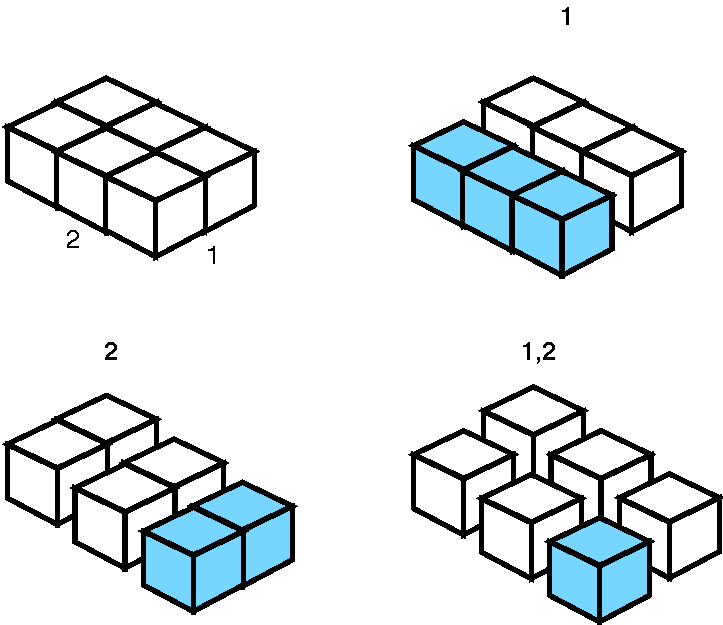
\includegraphics[width= 0.35 \textwidth]{input-a2}
  \caption{The four ways to split up a 2d matrix, labelled above by the dimensions that they slice up.  Original matrix shown at top left, with dimensions labelled.  Blue indicates a single piece of the output.}
  \label{fig:split-matrix}
\end{figure}

The 3d case is a little more complicated.  We have three 2d slices, three 1d slices, and one 0d slice.  These are shown in Figure~\ref{fig:split-array}.  Note how the pieces for the 1d slices correspond to the intersection of the 2d slices.  The margins argument works correspondingly for higher dimensions, with a combinatorial explosion in the number of possible ways to slice up the array, choose(slice-d, array-d), to be exact.

\begin{figure}[htbp]
  \centering
    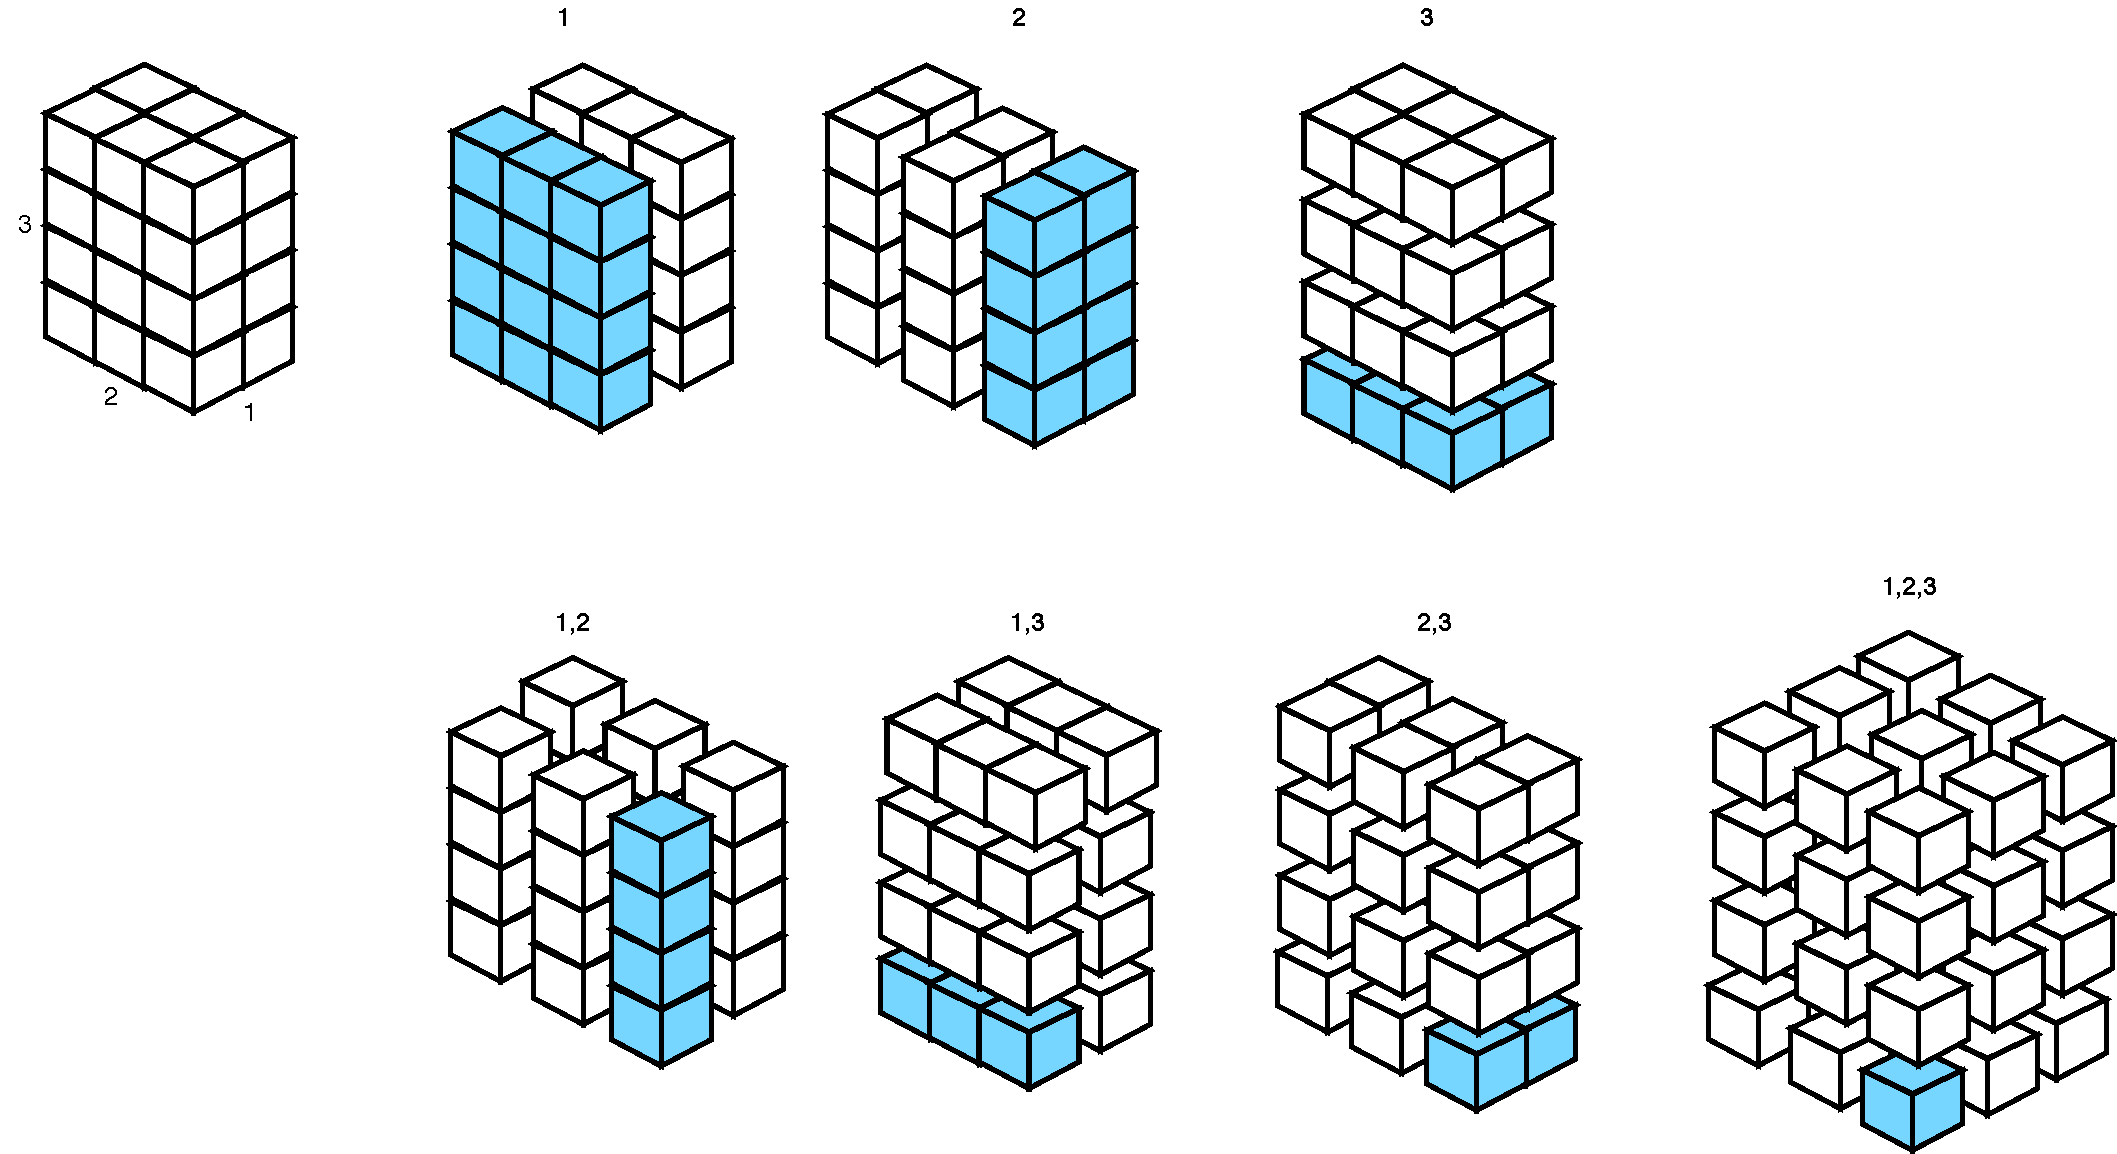
\includegraphics[width= \textwidth]{input-a3}
  \caption{The eight ways to split up a 3d array, labelled above by the dimensions that they slice up.  Original array shown at top left, with dimensions labelled.  Blue indicates a single piece of the output.}
  \label{fig:split-array}
\end{figure}

These default to working on the first dimension (i.e. row-wise) and automatically splat the function so that function is called not with a single list as input, but each column is passed as a separate argument to the function.  Compared to using {\tt mapply}, for the {\tt m*ply} functions you will need to {\tt cbind} the columns together first.  This will ensure that each argument has the same length, and allows the {\tt m*ply} functions to have the same argument order as all the other 

\paragraph{Special case: \code{m*ply}}  A special case of operating on arrays corresponds to the {\tt mapply} function of base R.  The plyr equivalents are named {\tt maply}, {\tt mdply}, {\tt mlply} and {\tt m\_ply}.  \f{mapply} takes multiple lists of parameters as input, and calls the processing function with a piece from each list as its parameters.  The input to \f{m*ply} is a little different: it is a list-array.


\subsubsection{Input: data frame ({\tt d*ply})}

When operating on a data frame, you usually want to split it up into groups based on combinations variables in the data set.  For {\tt d*ply} you specify   which variables (or functions of variables) to use.  These variables are specified in a special way to highlight that they are computed first from the data frame, then the global environment (in which case it's your responsibility to ensure that their length is equal to the number of rows in the data frame).  

\begin{itemize}
  \item \code{.(var1)} will split the data frame into groups defined by the value of the \code{var1} variable.  If you use multiple variables, {\tt .(a, b, c)}, the groups will be formed by the interaction of the variables, and output will be labelled with all three variables.  
  
  \item You can also use functions of variables: {\tt .(round(a))}, {\tt .(a * b)}.  If you are outputting to a data frame, these will get ugly names (produced by \f{make.names}), but you can override them by specifying names in the call: \code{.(product = a * b)}
  
  \item By default, \plyr will look in the data frame first, and then in the global environment {\tt .(anothervar)}.  However, you are encouraged to keep all related variables in the same data frame: this makes things much easier in the long run.
  
\end{itemize}

Figure~\ref{fig:split-data-frame} shows two examples of splitting up up a simple data frame.  Splitting up data frames is easier to understand (and to draw!) than splitting up arrays, because they're only 2 dimensional.

\begin{figure}[htbp]
  \centering
    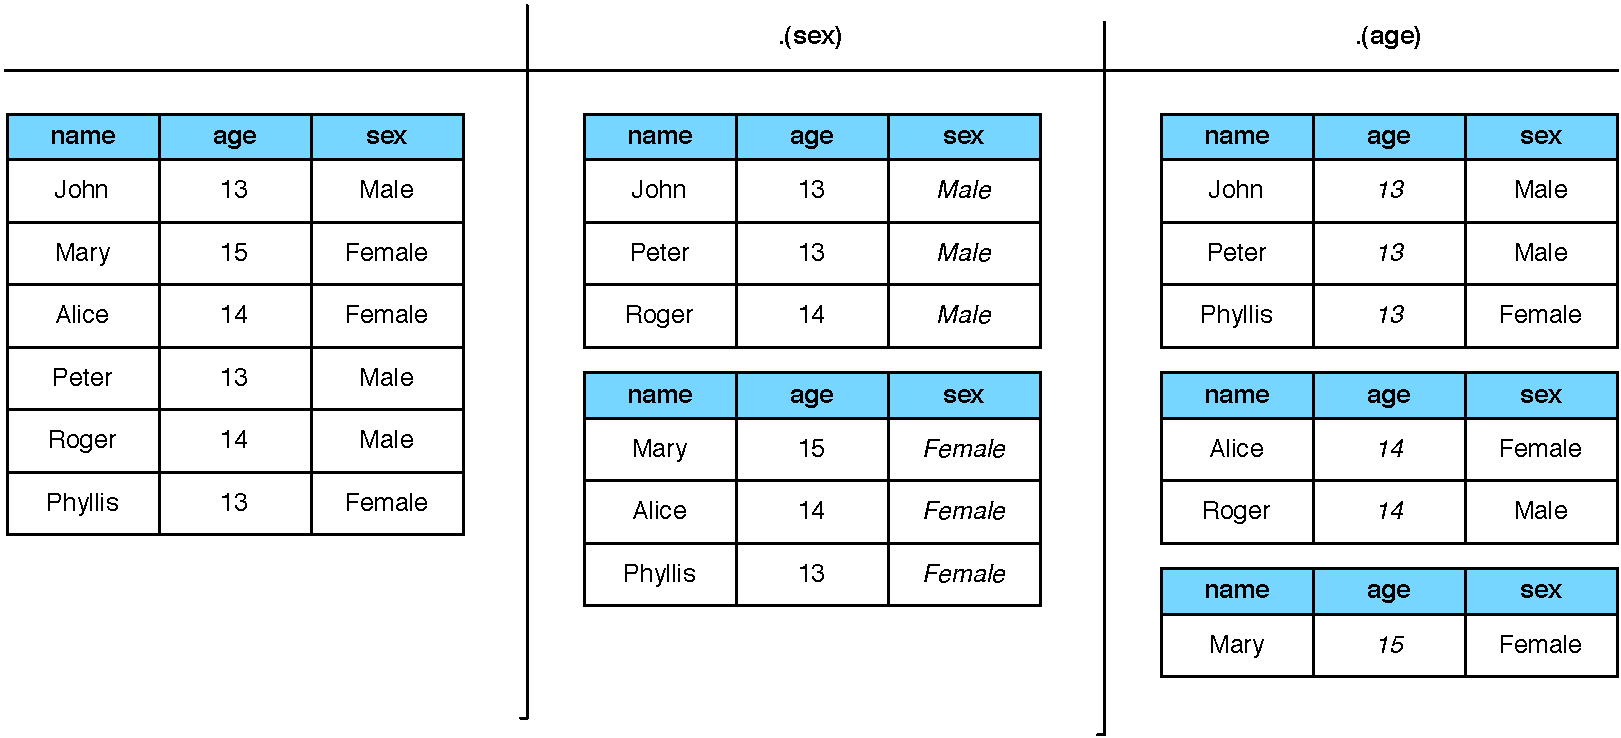
\includegraphics[width= \textwidth]{input-d}
  \caption{Two examples of splitting up a data frame by variables.  If the data frame was split up by both sex and age, there would only be one subset with more than one row: 13-year-old males.}
  \label{fig:split-data-frame}
\end{figure}


\subsubsection{Input: list (\code{l*ply})} 

Lists are the simplest type of input to deal with because they are already naturally divided into pieces: the elements of the list.  For this reason, the \code{l*ply} functions don't need an argument that describes how to break up the data structure.

\paragraph{Special case: \code{r*ply}}  A special case of operating on lists corresponds to \f{replicate} in base R, and is useful for drawing distributions of random numbers.  This is a little bit different to the other plyr methods.  Instead of the \code{data.} argument, it has \code{n.} the number of replications to run, and instead of a function it accepts a expression.  

\subsection{Output}
\label{sec:output}

The output type defines how the pieces will be joined back together again, and how they will be labelled.  The labels are particularly important to allow you to match up the input with the output.

The input and output types are the same, except there is an additional output option, which discard the output.  This is useful for functions with side effects that make changes outside of R

The output type also places some restrictions on what type of results the processing function should return.  Generally, the processing function should return the same type of data as the eventual output, (i.e.\ vectors, matrices and arrays for {\tt *aply} and data frames for {\tt *dply}) but some other formats are accepted for convenience and are described in Table~\ref{tbl:restrictions}.  These are explained in more detail in the individual output type sections.

\begin{table}
  \begin{center}
  \begin{tabular}{lll}
    \toprule
    Output & Processing function restrictions & Null output \\
    \midrule
     \code{*aply} & atomic array, or list & \f{logical} \\
     \code{*dply} frame  & data frame, or atomic vector & \f{data.frame}\\
     \code{*lply} & none & \f{list} \\
     \code{*_ply} & none &  \\
     \bottomrule  
  \end{tabular}
  \end{center}
  \caption{Summary of processing function restrictions and null output values for all output types.  Explained in more detail in each output section. }
  \label{tbl:restrictions}
\end{table}

% For any type, if the processing function returns {\tt NULL}, that slice will not be included in the output.

\subsubsection{Output: array ({\tt *aply})}

With array output the shape of the output array is determined by the input splits and the dimensionality of each individual result. Figures~\ref{fig:function-1d} and \ref{fig:function-2d} illustrate this pictorially for simple 1d and 2d cases.  For arrays, the pieces contribute to the output in the expected way; lists are related like a 1d array; and data frames get a dimension for each variable in the split.  The dimnames of the array will be the same as the input, if an array; or extracted from the subsets, if a data frame.

The processing function should return an atomic (i.e.\ logical, character, numeric or integer) array of fixed size/shape, or a list.  If atomic, the extra dimensions will added perpendicular to the original dimensions.  If a list, the output will be a list-array. If there are no results, {\tt *aply} will return a logical vector of length 0.  

All \code{*aply} functions have a \code{drop.} argument.  When this is true, the default, any dimensions of length one will be dropped.  This is useful because in R, a vector of length three is not equivalent to a 3\x1 matrix or a 3\x1\x1 array.

\begin{figure}[htbp]
  \centering
  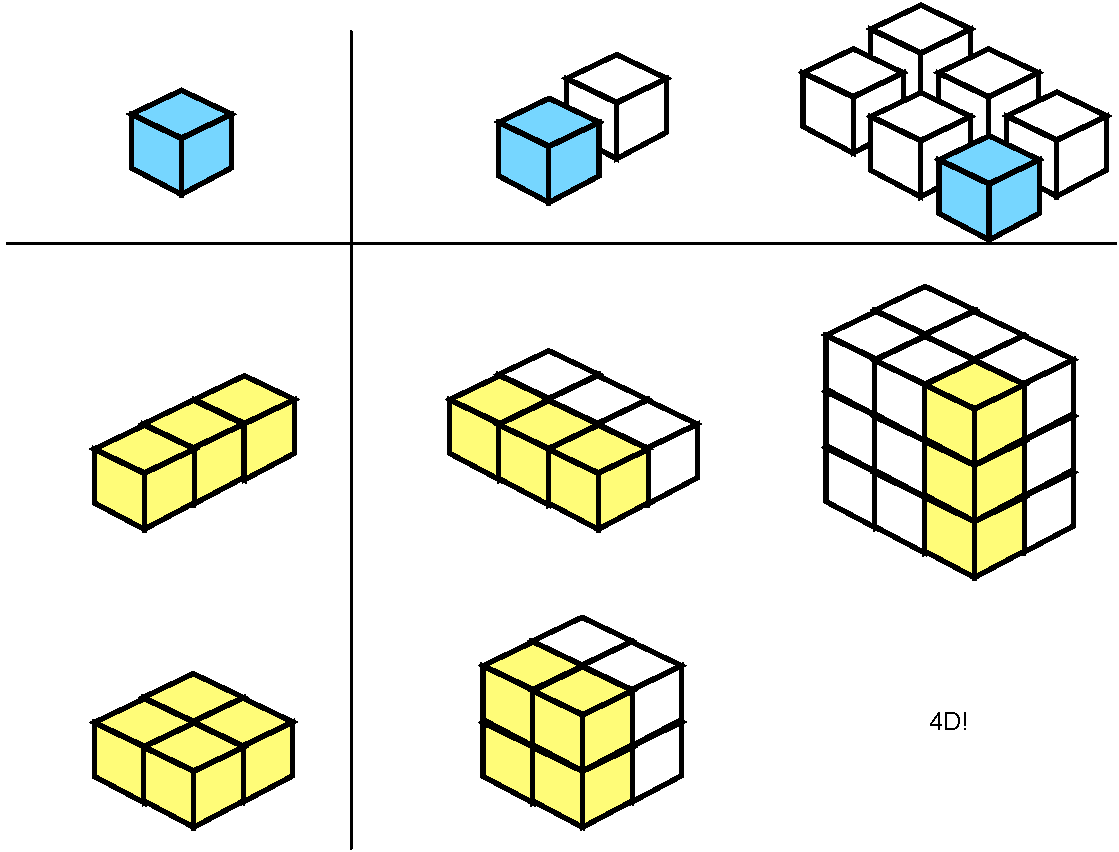
\includegraphics[width= 0.45 \textwidth]{output-a1}
  \caption{Results from outputs of various dimensionalty from a \textbf{single} value, shown top left.  Columns indicate input: (left) a vector of length two, and (right) a 2\x2 matrix.  Rows indicate the shape of a single processed piece: (top) a vector of length 3, (bottom) a 2\x2 matrix.  Extra dimensions are added perpendicular to existing ones.  The array in the bottom-right cell is 4d and so is not shown.}
  \label{fig:function-1d}
\end{figure}

\begin{figure}[htbp]
  \centering
  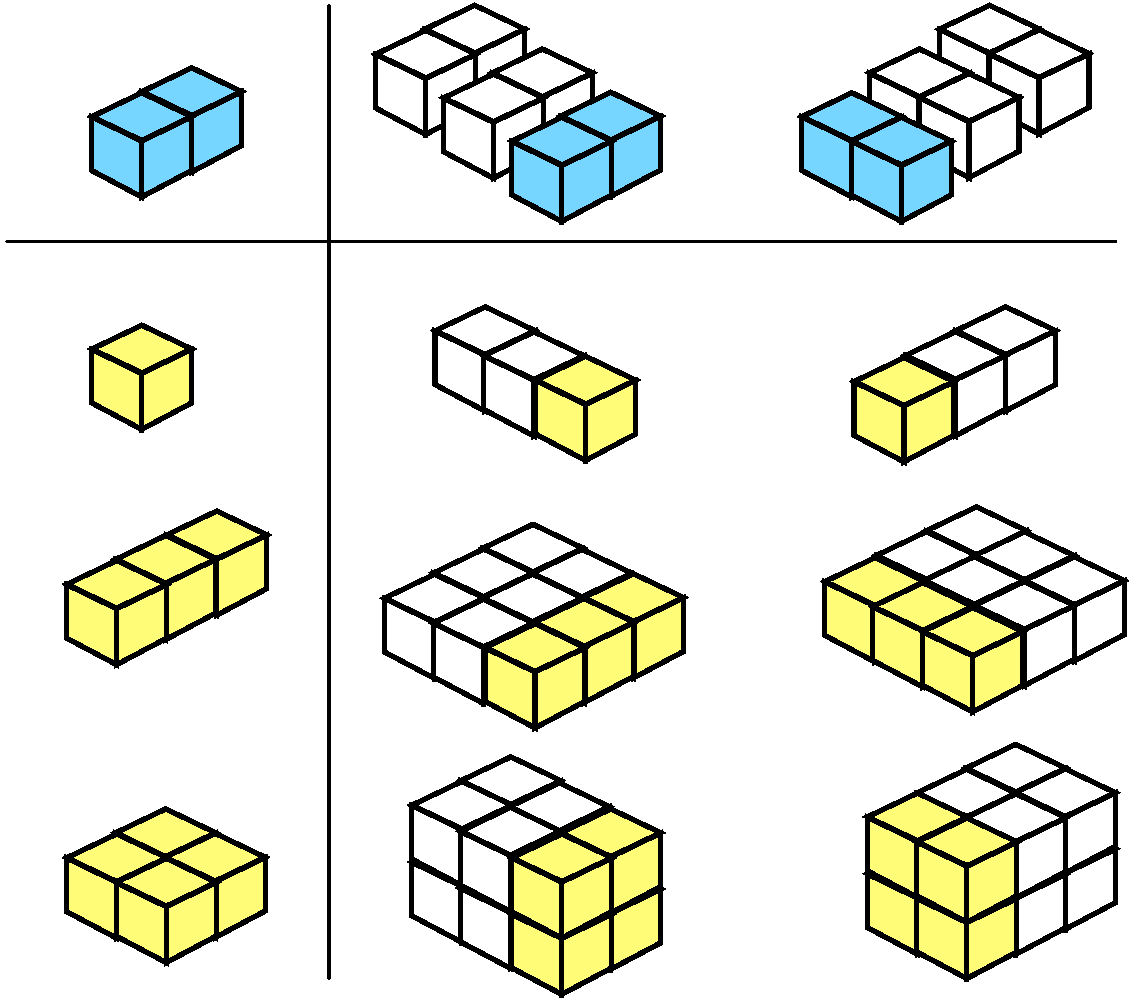
\includegraphics[width= 0.45 \textwidth]{output-a2}
  \caption{Results from outputs of various dimensionalty from a \textbf{1d vector}, shown top left.  Columns indicate input: (left) a 2\x3 matrix split by rows and (right) and 3\x2 matrix split by columns.  Rows indicate the shape of a single processed piece: (top) a single value, (middle) a vector of length 3, and (bottom) a 2\x2 matrix.}
  \label{fig:function-2d}
\end{figure}

\subsubsection{Output: data frames ({\tt *dply})}

When the output is a data frame, it will contain the results and additional columns that identify where in the original data each row came from.  These columns make it possible to merge the old and new data if you need to.  If the input was a data frame, there will be a column for variables used to split up the original data; if it was a list, a column for the names of the list; if an array, a column for the names of each splitting dimension.

The processing functions should either return a data.frame, or a (named) atomic vector of fixed length, which will form the columns of the output. If there are no results, {\tt *dply} will return an empty data frame.  \plyr provides an \code{as.data.frame} method for functions which can be handy: \code{as.data.frame(mean)} will create a new function which outputs a data frame.

\begin{figure}[htbp]
  \centering
    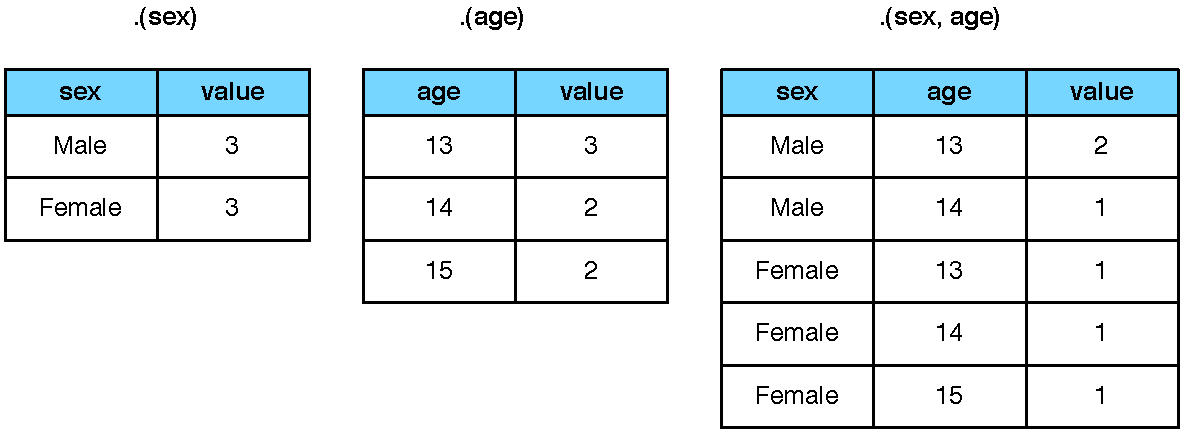
\includegraphics[width = 0.8 \textwidth]{output-d}
  \caption{Illustrating the output from using \f{ddply} on the example from Figure~\ref{fig:split-data-frame} with \f{nrow}.  Splitting variables shown above each example.  Note how the extra labelling columns are added so that you can identify to which subset the results apply.}
  \label{fig:label}
\end{figure}

\subsubsection{Output: list ({\tt *lply})}

This is the simplest output format, where each processed piece is joined together in a list.  The list also stores the labels associated with each pieces, so that if you use {\tt ldply} or {\tt laply} to further process the list the labels will appear as if you had used {\tt aaply}, {\tt adply}, {\tt daply} or {\tt ddply} directly.  {\tt llply} is convenient for calculating complex objects once (e.g.\ models), from which pieces of interest are later extracted into arrays and data frames.

There are no restrictions on the output of the processing function.  If there are no results, {\tt *lply} will return a list of length 0.

\subsection{Output: nothing ({\tt *\_ply})}

Sometimes you are operating on a list purely for the side effects (e.g. plots, caching, output to screen/file).  This is a little more efficient than abandoning the output of {\tt *lply} because it doesn't store the intermediate results.

\section{Helpers}
\label{sec:helpers}

The {\tt plyr} package also provides a number of helper function which take a function (or functions) as input and return a modified function as output.  

\begin{itemize}
  \item {\tt splat} converts a function to use.  This is useful when you want to pass a function a row of data frame or array, and don't want to manually pull it apart in your function.  For example:
  
  \begin{verbatim}
    hp_per_cyl <- function(hp, cyl, ...) hp / cyl
    splat(hp_per_cyl)(mtcars[1,])
    splat(hp_per_cyl)(mtcars)
  \end{verbatim} 
  
  Generally, splatted functions should have {\tt ...} as an argument, so you only need to specify the variables that you are interested in.  For more information on how splat works, see {\tt do.call}.  
  
  {\tt splat} is applied to functions used in {\tt m*ply} by default.

  \item {\tt each} takes a list of functions and produces a function that runs  each function on the inputs and returns a named vector of outputs.   For example, {\tt each(min, max)} is short hand for {\tt function(x) c(min = min(x), max = max(x))}.  Using each with a single function is useful if you want a named vector as output.

  \item {\tt colwise} converts a function that works on vectors, to one that operates column-wise of data frame, returning a data fram.  For example, {\tt colwise(median)} is a function that computes the median of each column of a data.frame.  
  
  The optional {\tt .if} argument specialises the function to only run on certain types of vector, e.g.\ {\tt .if = is.factor} or {\tt .if = is.numeric}.  These two restrictions are provided in the premade {\tt calcolwise} and {\tt numcolwise}.  
  
  \item {\tt failwith} sets a default value to return if the function throws an error.  For example, {\tt failwith(NA, f)} will return an {\tt NA} whenever {\tt f} throws an error.  
  
  The optional {\tt quiet} argument suppresses any notice of the error when it is {\tt TRUE}.

\end{itemize}

Each plyr function also has a {\tt progress.} argument which allows you to monitor the progress of long running operations.  There are four difference progress bars:

\begin{itemize}
  \item {\tt "none"}, the default.  No progress bar is displayed.
  \item {\tt "text"} provides a textual progress bar which.
  \item {\tt "win"} and {\tt "tk"} provide graphical progress bars for Windows and systems with the tcl/tk package loaded.
\end{itemize}

The progress bars assume that processing each piece takes the same amount of time, so will not be 100\% accurate.

\section{Strategy}
\label{sec:strategy}



\begin{enumerate}
  \item Extract a subset of the data for which it is easy to solve the problem
  \item Solve the problem by hand, checking as you go
  \item Write a function that encapsulates the solution
  \item Use the appropriate ply function to split up the original data, apply the function and join the pieces back together.
  
\end{enumerate}

The following two case studies illustrate these techniques for a range of problems related to a data frame storing the batting records for long-term baseball players, and a 3d array representing space and time values of ozone.

\subsection{Case study: baseball}

The {\tt baseball} data set contains the batting records for all professional US players with 15 or more years of data.  The complete list of variables are described fully {\tt ?baseball}, but for this example we will focus on just four: {\tt id}, which identifies the player, {\tt year} the year of the record and {\tt rbi} the number of runs that the player made in the season, and {\tt} at bat, the number of times the player had an opportunity to hit the ball.

(This is a rather crude analysis, as it doesn't take into account the people that might already be on the other plates)

What we'll explore is the performance of a batter over his career.  To get started, we need to calculate the careeryear, i.e. the number of years since the player started playing.  This is easy to do if we have a single player:

\begin{verbatim}
baberuth <- subset(baseball, id == "ruthba01")
baberuth$cyear <- baberuth$year - min(baberuth$year) + 1
\end{verbatim}

To do this for all players, we first make a function:

\begin{verbatim}
calculate_cyear <- function(df) {
  transform(df, 
    cyear = year - min(year),
    cpercent = (year - min(year)) / (max(year) - min(year))
  )
}
\end{verbatim}

\noindent and then split up the whole data frame into people, run the function on each piece and join them back together into a data frame:

% qplot(ab, data=baseball, geom="histogram", binwidth=10)
% qplot(ab, data=subset(baseball, ab < 100), geom="histogram", binwidth=5)

\begin{verbatim}
baseball <- ddply(baseball, .(id), calculate_cyear)
baseball <- subset(baseball, ab >= 25)
\end{verbatim}

% qplot(cyear, rbi / ab, data=baseball, group=id, geom="line", colour=I(alpha("black", 1/20)))

To summarise the pattern across all players, we first need to figure out what the common patterns are.  A time series plot of rbi/ab, runs per bat, is a good place to start.  We do this for Babe Ruth, as shown in Figure~\ref{fig:baberuth}, then write a function to do it for any player (taking care to ensure common scale limits) and then use {\tt d\_ply} to save a plot for every player to a pdf.  We use two tricks here: {\tt reorder} to sort the players in order of average rbi / ab, and {\tt failwith} to ensure that even if a single plot doesn't work we will still get output for the others.

\begin{figure}[htbp]
  \centering
    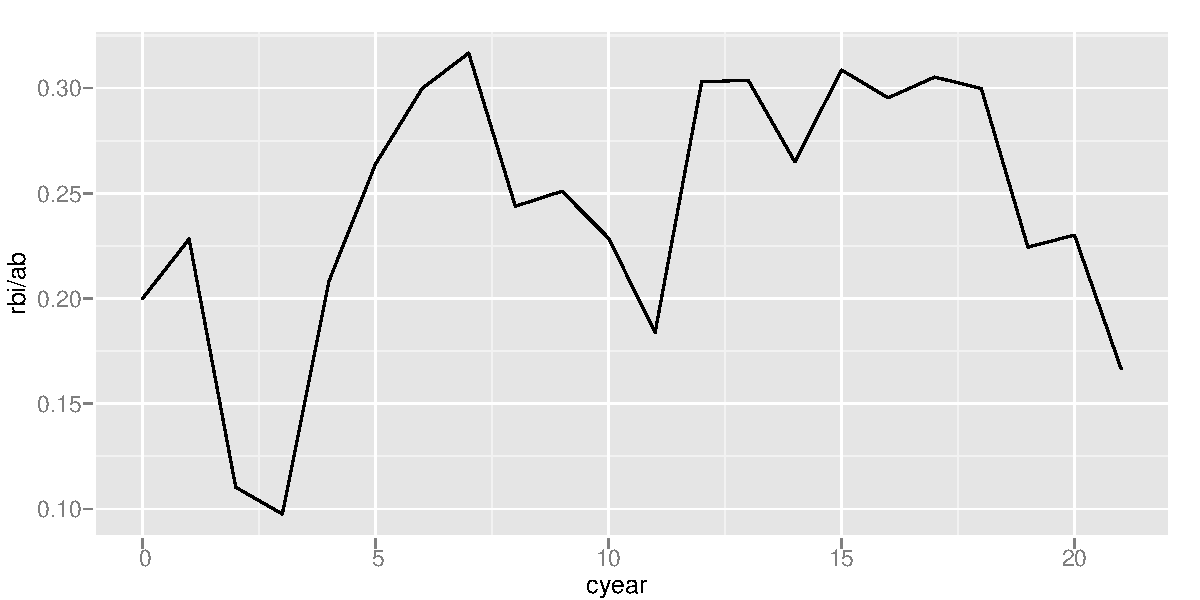
\includegraphics[width=3in]{baberuth}
  \caption{Runs per bat for Babe Ruth.}
  \label{fig:baberuth}
\end{figure}

\begin{verbatim}
qplot(cyear, rbi / ab, data=baberuth, geom="line")  

xlim <- range(baseball$cyear, na.rm=TRUE)
ylim <- range(baseball$rbi / baseball$ab, na.rm=TRUE)
plotpattern <- function(df) {
  print(qplot(cyear, rbi / ab, data = df, geom="line", xlim = xlim, ylim = ylim ))
}

pdf("paths.pdf", width=8, height=4)
d_ply(baseball, .(reorder(id, rbi / ab)), failwith(NA, plotpattern))
dev.off()
\end{verbatim}

Flicking through the 1145 plots reveals that there doesn't seem to be much of a common pattern, although many players do seem to have a roughly linear trend with quite a bit of noise.  We'll start by fitting a linear model to each player and then exploring the results.  This time we'll skip doing it by hand and go directly to the function.

\begin{verbatim}
model <- function(df) {
  lm(rbi / ab ~ cyear, data=df)
}
model(baberuth)
models <- dlply(baseball, .(id), model)
\end{verbatim}

Now we have a list of 1145 models, one for each player.  To do something interesting with these, we need to extract some summary statistics.  We'll extract the coefficients of the model (the slope and intercept), and a measure of model fit so we can ensure we're not drawing conclusions based on models that fit the data very poorly, the R-squared.  The first few rows of {\tt coef} are shown in Table~\ref{tbl:coef}.

\begin{verbatim}
rsq <- function(x) summary(x)$r.squared
coef <- ldply(models, function(x) c(coef(x), rsq(x)))
names(coef) <- c("id", "intercept", "slope", "rsquare")
\end{verbatim}

\begin{table}[ht]
  \centering
  \begin{tabular}{lrrr}
    \hline
    id & intercept & slope & rsquare \\
    \hline
    aaronha01 & 0.18 & 0.00 & 0.00 \\
    abernte02 & 0.00 &  & 0.00 \\
    adairje01 & 0.09 & $-$0.00 & 0.01 \\
    adamsba01 & 0.06 & 0.00 & 0.03 \\
    adamsbo03 & 0.09 & $-$0.00 & 0.11 \\
    adcocjo01 & 0.15 & 0.00 & 0.23 \\
    \hline
  \end{tabular}
  \caption{The first few rows of the {\tt coef} data frame.  Note that the player ids from the original data have been preserved}
  \label{tbl:coef}
\end{table}

Figure~\ref{fig:models-hist} displays the distribution of r-squared across the models.  The models generally do a very bad job of fitting the data!  
Figure~\ref{fig:models} summarises these bad models.  These plots show a negative correlation between slope and intercept, and the particularly bad models have estimates for both values close to 0.  Reassuringly, there are no players in the bottom left quadrant with both negative slope and intercept.

% qplot(rsquare, data=coef, geom="histogram", binwidth=0.01)
% ggsave(file = "models-hist.pdf", width=12, height=4)
\begin{figure}[htbp]
  \centering
    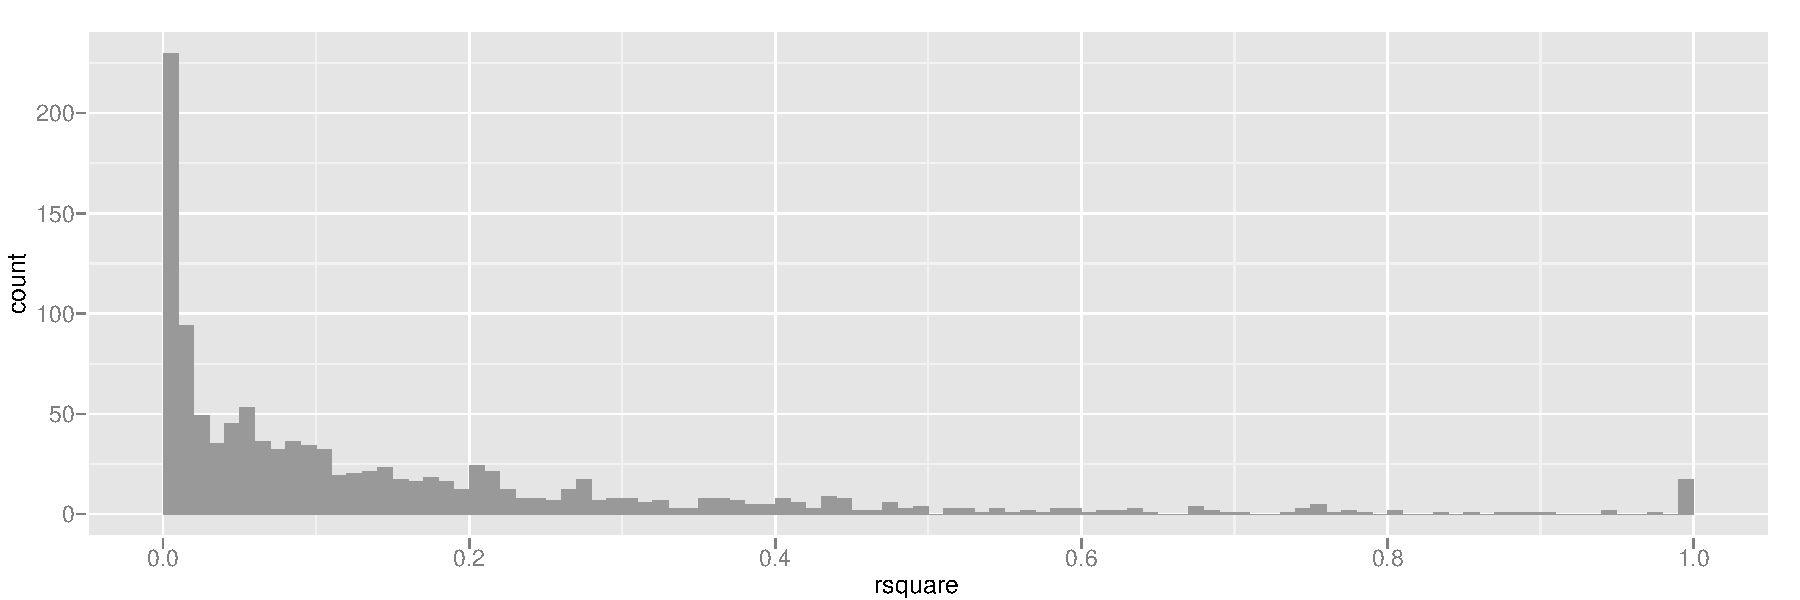
\includegraphics[width=\textwidth]{models-hist}
  \caption{Histogram of model r-squared with bin width of 0.05.  Most models fit very poorly!  The spike of models with a r-squared of 1 are players with only two data points, found by inspecting {\tt ldply(models[coef\$rsquare == 1], "[[", "model")}}
  \label{fig:models-hist}
\end{figure}

% ggplot(coef, aes(slope, intercept)) + 
%   geom_point(aes(size = rsquare)) +
%   geom_vline(size=0.5, colour="grey50") + 
%   geom_hline(size = 0.5, colour="grey50") + 
%   scale_area()
% ggsave(file = "models.pdf", width=6, height=6)
% last_plot() + xlim(-0.01, 0.01) + ylim(-0.1, 0.25)
% ggsave(file = "models-zoom.pdf", width=6, height=6)
\begin{figure}[htbp]
  \centering
    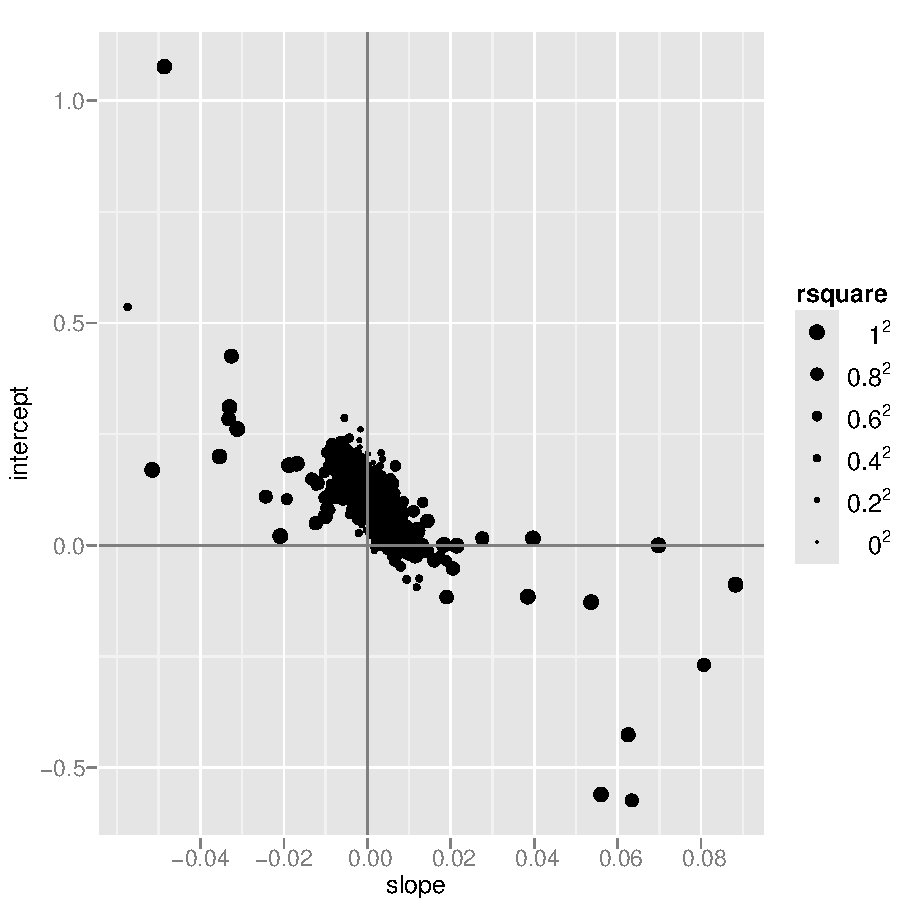
\includegraphics[width=0.5\textwidth]{models}%
    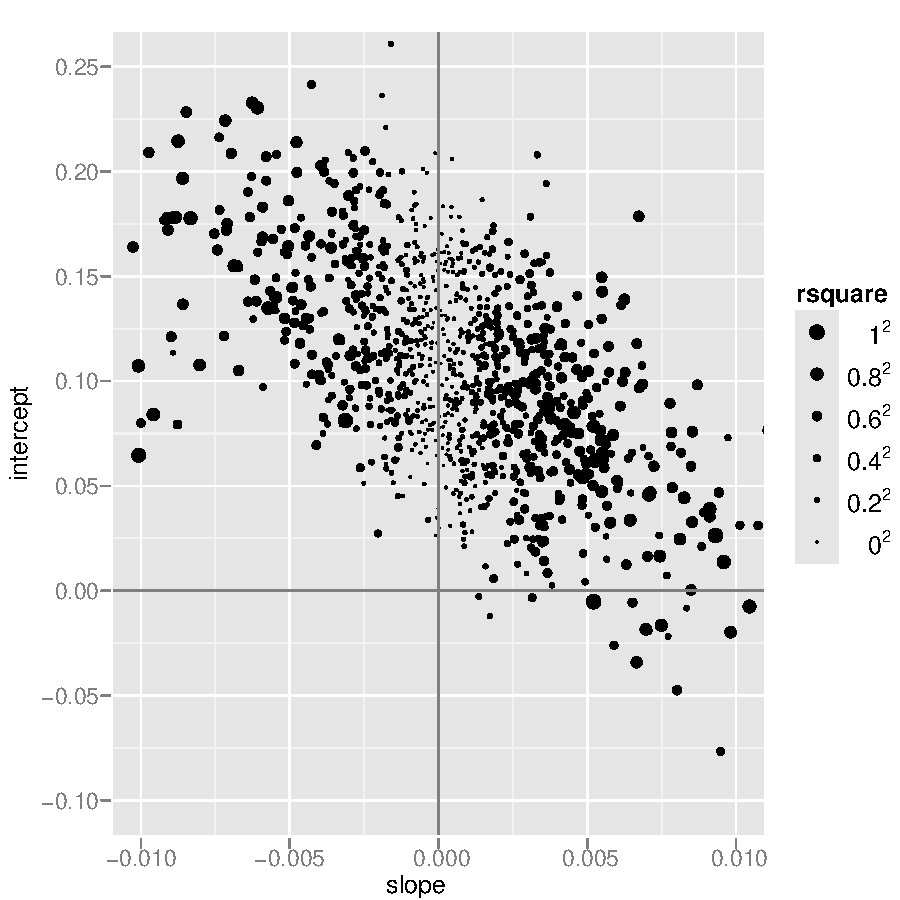
\includegraphics[width=0.5\textwidth]{models-zoom}
  \caption{A scatterplot of model intercept and slope, with one point for each model (player).  The size of the points is proportion to the R-square of the model. Vertical and horizontal lines emphasis the x and y origins. }
  \label{fig:models}
\end{figure}

This concludes the baseball player case study, which used used {\tt ddply}, {\tt d\_ply}, {\tt dlply} and {\tt ldply}.  Our statistical analysis was not very sophisticated, but the tools of {\tt plyr} made it very easy to work at the player level, and then combine results into a single summary.  

\subsection{Case study: ozone}
\label{sub:ozone}

In this case study we will analyse a 3d array that records ozone levels over a 24\x24 spatial grid at 72 time points \citep{hobbs:2007}.  This produces a 24\x24\,$times$\,72 3d array, containing a total of 41\,472 data points.  Figure~\ref{fig:ozone-glyph} is one way of displaying this data.  Conditional on spatial location, each glyph shows the evolution of ozone levels for each of the 72 months (6 years).  The striking seasonal patterns make it difficult to see if there are any long-term changes.  In this case study, we will explore how to separate out and visualise the seasonal effects.

\begin{figure}[htbp]
  \centering
    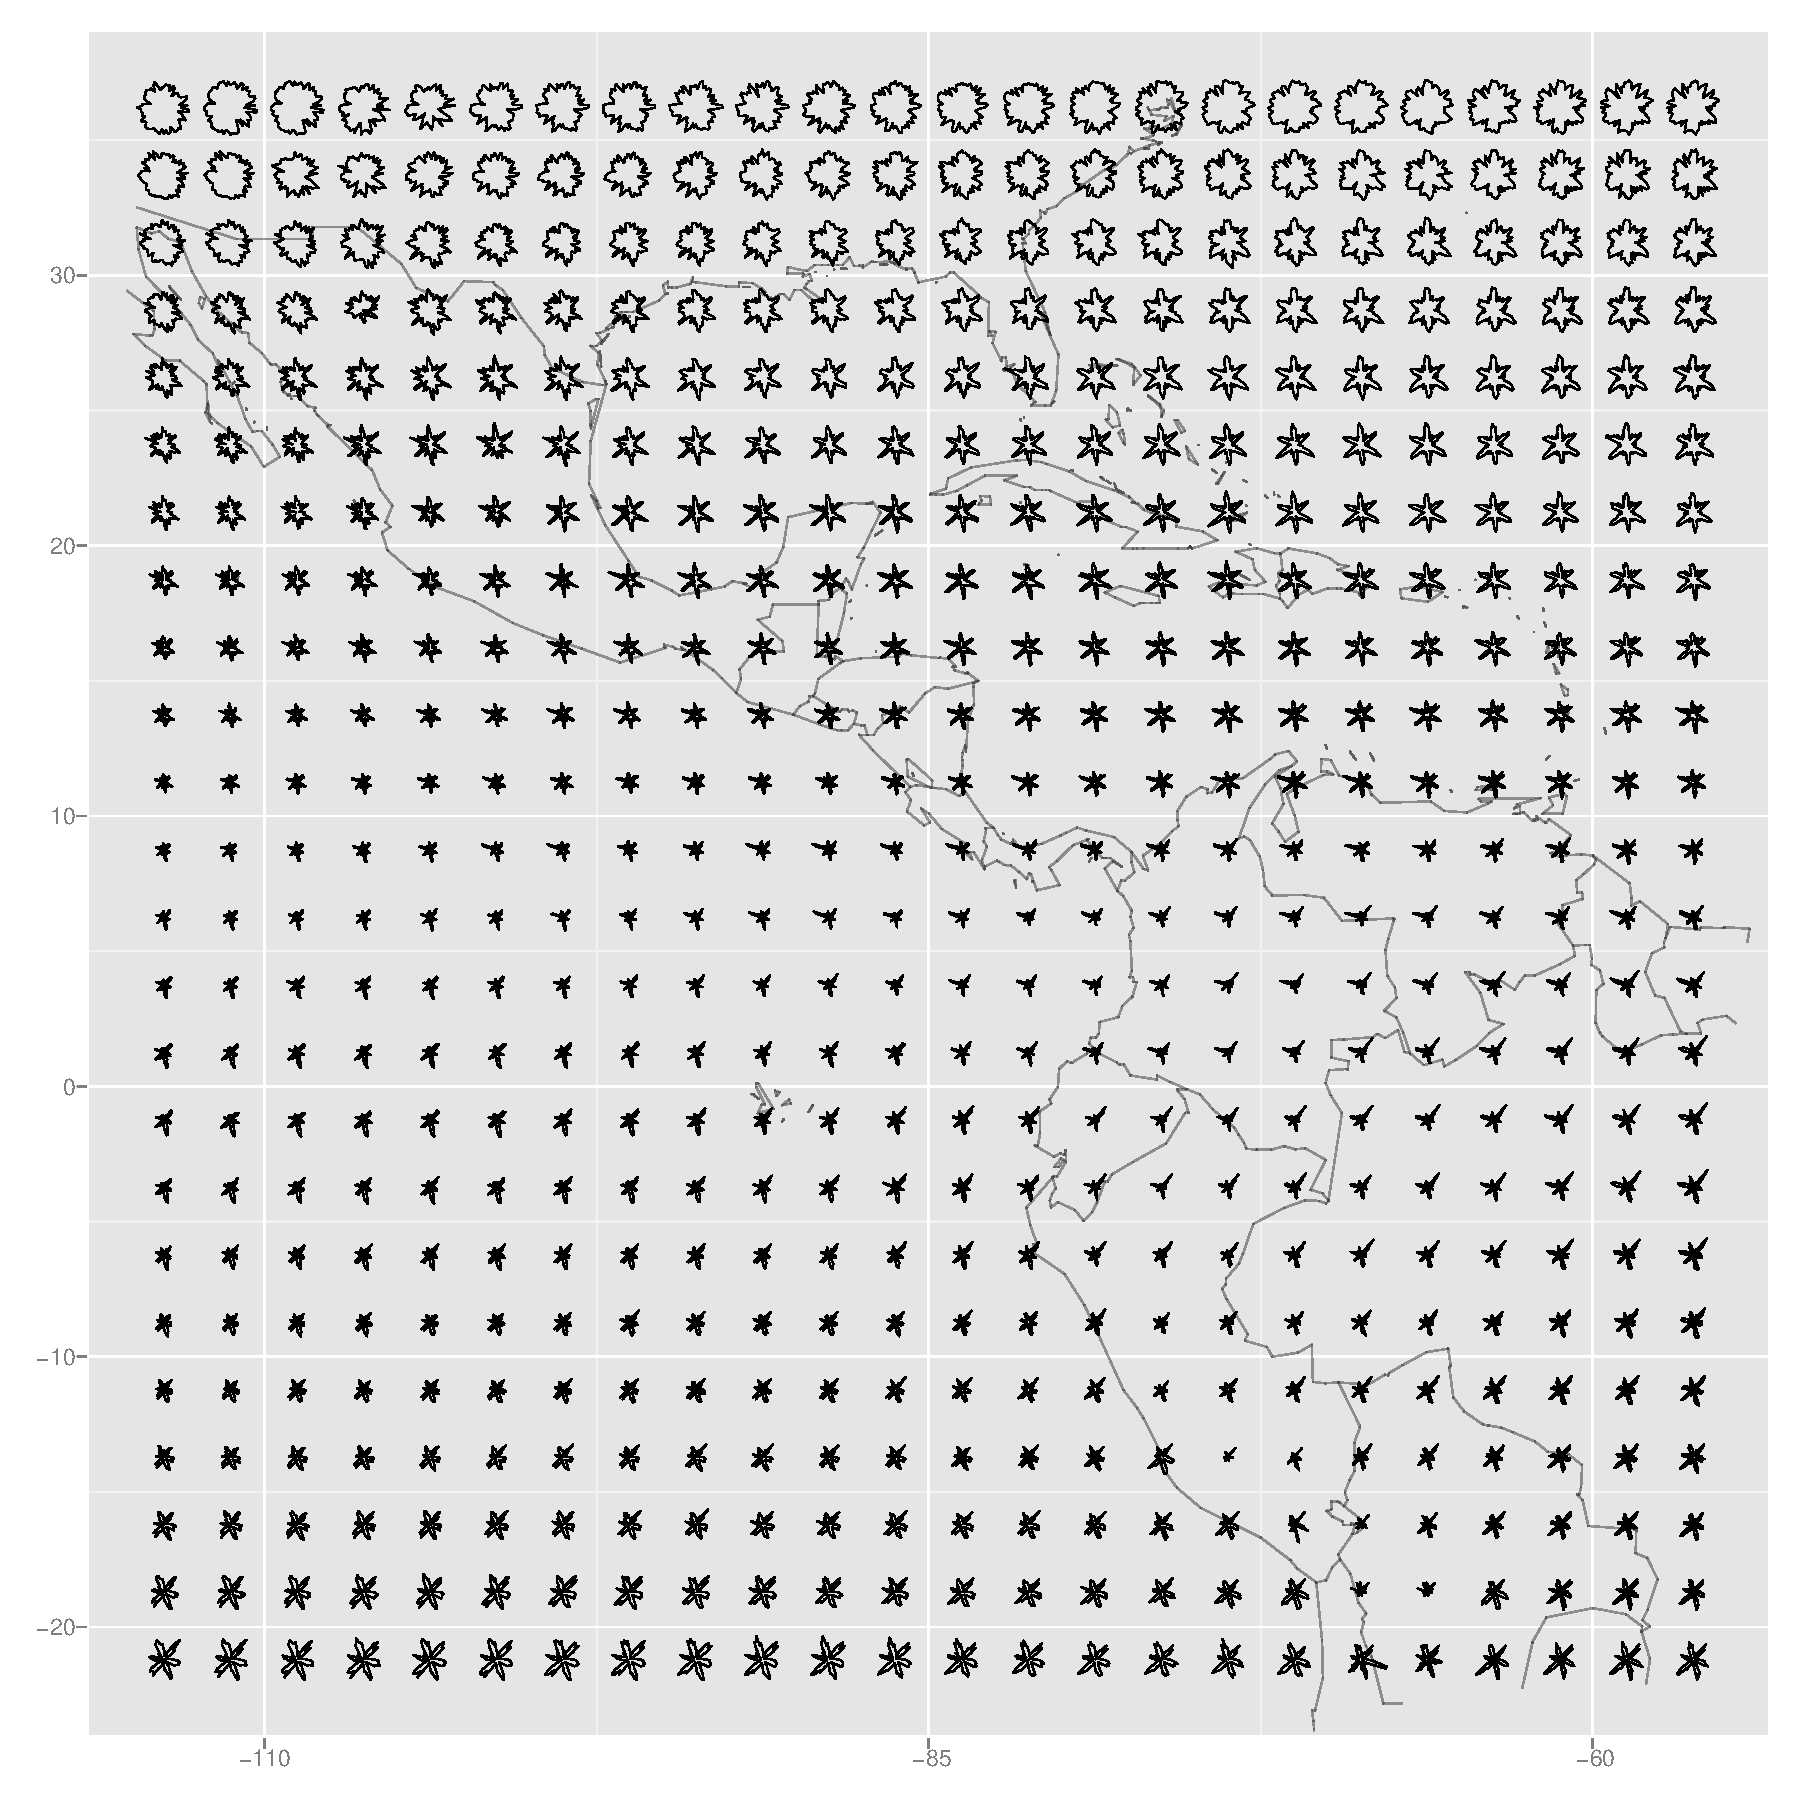
\includegraphics[width=4in]{ozone-glyph}
  \caption{Star glyphs showing variation in ozone over time at each spatial location.}
  \label{fig:ozone-glyph}
\end{figure}

Again we will start with the simplest case: a single time point, from location (1, 1).  Figure~\ref{fig:ozone-ts} displays this in two ways: as a single line over time, or a line for each year over the months.  This second plot illustrates the striking seasonal variation at this time point.

% INTERWEAVE
% 
% value <- ozone[1, 1, ]
% time <- 1:72
% month.abbr <- c("Jan", "Feb", "Mar", "Apr", "May", 
%  "Jun", "Jul", "Aug", "Sep", "Oct", "Nov", "Dec")
% month <- factor(rep(month.abbr, length = 72), levels = month.abbr)
% year <- rep(1:6, each = 12)
\input{_include/c2d71cd30a5f537fc57fe5350efb948c.tex}
% END

% FIGURE
%  LABEL: ozone-ts 
%  CAPTION: Two ways of displaying the seasonal changes.  (Left) A single time
%  series over all six years and (right) a line for each year.
% 
% qplot(time, value, geom="line")
% qplot(month, value, geom="line", group = year)
\input{_include/f175a54909fe54e7ce00a2a6823c75c5.tex}
% END

We are going to use a quick and dirty method to remove the season variation: we'll look at the residuals from a robust linear model, predicting amount of ozone by month.  We also need to create a few time related variables:

% INTERWEAVE
% 
% library(MASS)
%
% deseas <- rlm(value ~ month - 1)
\input{_include/db58b8c3031d9ed8726a9842095330f6.tex}
% END

% FIGURE
%  LABEL: ozone-ts-desas
%  CAPTION: Deasonalised ozone trends.  (Left) deasonalised trend over 
%  six years.  (Right) Estimates of seasonal effects.  Compare to
%  Figure~\ref{fig:ozone-ts}
%
% qplot(time, resid(deseas), geom="line")
% qplot(month, unname(coef(deseas)), geom="line", group = 1)
\input{_include/d7b07b226f5f0abde882229141f50eb1.tex}
% END

We next turn this into a function and apply fit model to all of the spatial locations.  This does take a little while, but we are fitting 576 models!  From those models we extract the deasonalised values (the residuals) and the seasonal coefficients.  Looking at the dimensionality we see that they're in the same format as the original data.

% INTERWEAVE
% 
% deseasf <- function(value) rlm(value ~ month - 1)
% 
% models <- alply(ozone, 1:2, deseasf)
% coefs <- laply(models, coef)
% dimnames(coefs)[[3]] <- months.abbr
% names(dimnames(coefs))[3] <- "month"
% 
% deseas <- laply(models, resid)
% dimnames(deseas)[[3]] <- 1:72
% names(dimnames(deseas))[3] <- "time"
% 
% dim(coefs)
% dim(deseas)

Figure~\ref{fig:glyph-deseas} and Figure~\ref{fig:glyph-coef} visualises these results with star glyph plots.  For plotting, it's more convenient to have the data in data frames.  There are few different ways to do this: we can convert from the 3d array to a data frame with \f{melt} from the reshape package, or use \f{ldply} instead of \f{laply}.  For this example, we'll use a combination of these techniques.  We'll convert the original array to a data frame, add on some useful columns, and then perform the same steps as above with this new format.

% INTERWEAVE 
% 
% coefs_df <- melt(coefs)
% levels(coefs_df$month) <- month.abbr
% head(coefs_df)
% deseas_df <- melt(deseas)
% head(deseas_df)

\begin{verbatim}
source("ozone-map.r")

res <- 1.5
coef_stars <- oz_stars(coefs_df, "month", "value")
ggplot(coef_stars, aes(x = long + res * x, y = lat + res * y)) + map + geom_polygon(aes(group = interaction(long, lat)), fill=NA, colour="black")

qplot(month, value, data=coefs_df, geom="line", group=interaction(lat,long))
qplot(long, lat, data=subset(coefs_df, month =="Jan"), fill = value, 
geom="tile") + map

qplot(long, lat, data=subset(coefs_df, month =="Jan"), size = value) + scale_area(to=c(2,6))

coef_limits <- range(coef2$coef)
coef_mid <- mean(coef2$coef)
monthsurface <- function(mon) {
  df <- subset(coef2, month == mon)
  qplot(long, lat, data = df, fill = coef, geom="tile", main = mon) + 
  scale_fill_gradient2(limits = coef_limits, midpoint = coef_mid) + map
}

pdf("~/desktop/ozone-animation.pdf", width=8, height=8)
l_ply(month.abbr, monthsurface, print. = TRUE)
dev.off()

seassum <- ddply(coef2, .(lat, long), function(df) {
  each(mean, sd)(df$coef)
})
qplot(long, lat, data=seassum, fill = sd, geom="tile")
qplot(long, lat, data=seassum, fill = mean, geom="tile")
qplot(mean, sd, data=seassum)
\end{verbatim}

\begin{verbatim}
ozm <- melt(deseas)
names(ozm) <- c("lat", "long", "time", "value")
ozm[1:2] <- llply(ozm[1:2], function(x) as.numeric(as.character(x)))

small_mult(ozm) + geom_line(aes(group = interaction(lat,long)))

ozm <- melt(coef2)
ozm[1:2] <- llply(ozm[1:2], function(x) as.numeric(as.character(x)))
ozm$time <- as.numeric(ozm$month)

small_mult(ozm) + geom_line(aes(group = interaction(lat,long)))

\end{verbatim}

For many other types of operations, it is useful to convert this array structure to a data frame.  The {\tt melt} function in the {\tt reshape} package is one way to do that which preserves the dimension labels as much as possible.  If the data is this format we need few changes to the above code:

\begin{verbatim}
library(reshape)
ozonem <- melt(ozone)

models <- dlply(ozone, .(lat, long), deasf)
coefs <- ldply(models, coef)
deseas <- ldply(models, resid)

\end{verbatim}

This is the power of plyr: you don't need to worry about whether your data is a list, data frame or array, you can use whatever feels most natural.

\subsection{Other uses}

Randomisation within groups.  Simulation.

\section{Equivalence to existing R functions}
\label{sec:equiv}

Table~\ref{tbl:equiv} describes the equivalent between functions in base R and 
the functions provided by {\tt plyr}.  The built in R functions focus mainly on arrays and lists, not data frames, and most provide an argument to determine whether an array or list should be returned.  The syntax is also less consistent than plyr, for example, {\tt mapply} takes a function as the first argument rather than the input data.  Compared to {\tt apply}, {\tt aaply} returns the dimensions in a different order so as to be idempotent - i.e.\ {\tt apply(x, a, function(x) x) == x} for all {\tt a}. 

Avoid any ambiguity about what you'll get back from one of these functions. This replaces the {\tt simplify} argument that many of the {\tt apply} functions in base R has, and means that you can depend on the output of each function being a given type (which makes programming with the results easier).


\begin{table}[htpb]
  \begin{center}
  \begin{tabular}{llll}
    \toprule
    base & from & to & plyr \\
    \midrule
    \code{apply }    & a & a   & \code{aaply} \\
    \code{lapply}    & l & l   & \code{llply} \\
    \code{sapply}    & l & a   & \code{laply} \\
    \code{mapply}    & a & a/l & \code{maply} / \code{mlply} \\
    \code{by}        & d & l   & \code{dlply} \\
    \code{aggregate} & d & d   & \code{ddply} + \code{colwise} \\
    \bottomrule
  \end{tabular}
  \end{center}
  \caption{Mapping between apply functions and plyr functions.}
  \label{tbl:equiv}
\end{table}

Related functions {\tt tapply}, {\tt ave} and {\tt sweep} have no corresponding function in {\tt plyr}, and still remain useful. {\tt merge} is also for combining summaries with the original data.  The cast function in the reshape package \citep{reshape} is closely related to {\tt aaply}.

There are a number of other resources that also attempt to simplify this class of problems:

\begin{itemize}
  \item The {\tt doBy} package
  \item The {\tt gdata} package
  \item The {\tt scope} package
  \item Data manipulation in R, by Phil Spector
  \item Chapters in MASS, R intro?
  
\end{itemize}

\section{Future plans}
\label{sec:future}

If slow, might want to look at the profr package to speed up.  

However, it is my aim to eventually implement these functions in C for maximum speed and memory efficiency, so that they are competitive with the built in operations.  I also plan to investigate a connection to the {\tt papply} function to allow for easy parallelisation across multiple instances of R (particularly for multi-core machines).

multir

\bibliography{/Users/hadley/documents/phd/references}
\end{document}
